\documentclass{oblivoir}
\usepackage{amsmath,amssymb,amsthm,kotex,paralist,kswrapfig,graphicx}

\usepackage[skipabove=10pt,innertopmargin=10pt]{mdframed}

\usepackage{tabto,pifont}
\TabPositions{0.2\textwidth,0.4\textwidth,0.6\textwidth,0.8\textwidth}
\newcommand\tabb[5]{\par\bigskip\noindent
\ding{172}\:{\ensuremath{#1}}
\tab\ding{173}\:\:{\ensuremath{#2}}
\tab\ding{174}\:\:{\ensuremath{#3}}
\tab\ding{175}\:\:{\ensuremath{#4}}
\tab\ding{176}\:\:{\ensuremath{#5}}}

\usepackage{enumitem}
\setlist[enumerate]{label=(\arabic*)}

\newcounter{num}
\newcommand{\defi}[1]
{\noindent\refstepcounter{num}\textbf{정의 \arabic{num}) #1}\par\noindent}
\newcommand{\theo}[1]
{\noindent\refstepcounter{num}\textbf{정리 \arabic{num}) #1}\par\noindent}
\newcommand{\exam}[1]
{\bigskip\bigskip\noindent\refstepcounter{num}\textbf{예시 \arabic{num}) #1}\par\noindent}
\newcommand{\prob}[1]
{\bigskip\bigskip\noindent\refstepcounter{num}\textbf{문제 \arabic{num}) #1}\par\noindent}
\newcommand{\proo}
{\bigskip\textsf{증명)}\par}

\newcommand{\ans}{
{\par
\raggedleft\textbf{답 : (\qquad\qquad\qquad\qquad\qquad\qquad)}
\par}\bigskip\bigskip}

\newcommand{\pb}[1]%\Phantom + fBox
{\fbox{\phantom{\ensuremath{#1}}}}

\newcommand\ba{\,|\,}

\newcommand\an[1]{\par\bigskip\noindent\textbf{문제 #1)}\\}

\let\oldsection\section
\renewcommand\section{\clearpage\oldsection}

%%%%
\begin{document}

\title{윤영 : 07 집합(2)}
\author{}
\date{\today}
\maketitle
\tableofcontents
\newpage

%%

%%
\section{집합의 연산}
\begin{mdframed}
%
\defi{교집합과 합집합}
집합 \(A\)와 \(B\)에 대해, 두 집합에 공통적으로 들어있는 원소들로 이루어진 집합을 `\(A\)와 \(B\)의 \textbf{교집합}'이라고 하고, 기호로
\[A\cap B\]
로 쓴다.
또, 두 집합 중 하나에라도 속해있는 원소들로 이루어진 집합을 `\(A\)와 \(B\)의 \textbf{합집합}'이라고 하고, 기호로
\[A\cup B\]
라고 쓴다.
조건제시법으로 표현하면
\begin{align*}
A\cap B&=\{x\ba x\in A\text{ 그리고 }x\in B\}\\
A\cup B&=\{x\ba x\in A\text{ 혹은 }x\in B\}
\end{align*}
이고, 벤다이어그램으로 표현하면
\vspace{20pt}
\begin{center}
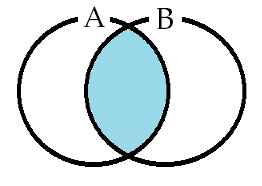
\includegraphics[width=0.3\textwidth]{intersection}~
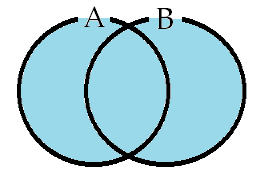
\includegraphics[width=0.3\textwidth]{union}

\(A\cap B\qquad\qquad\qquad\qquad A\cup B\)
\end{center}
이다.
\end{mdframed}

\kswrapfig[Pos=r]{union_and_intersection}{
%
\exam{}
두 집합 \(A=\{2,3,5,7\}\), \(B=\{1,2,3\}\)에서
\begin{align*}
A\cap B&=\{2,3\}\\
A\cup B&=\{1,2,3,5,7\}
\end{align*}
}

%
\prob{}
다음 두 집합 \(A\), \(B\)에 대하여 \(A\cap B\)와 \(A\cup B\)를 구하여라.
\begin{enumerate}
\item
\(A=\{x\ba x\text{는 6의 약수}\}\), \tabto{0.48\textwidth}
\(B=\{x\ba x\text{는 10보다 작은 소수}\}\)
\par\noindent
\(A\cap B=\)
\par\noindent
\(A\cup B=\)
\item
\(A=\{x\ba1\le x\le10,\:x\text{는 홀수}\}\), \tabto{0.48\textwidth}
\(B=\{2,5,8\}\)
\par\noindent
\(A\cap B=\)
\par\noindent
\(A\cup B=\)
\item
\(A=\{x\ba-3\le x\le4\}\), \tabto{0.48\textwidth}
\(B=\{x\ba1<x<9\}\)
\par\noindent
\(A\cap B=\)
\par\noindent
\(A\cup B=\)
\end{enumerate}

\clearpage
\begin{mdframed}
%
\defi{여집합과 차집합}
\textbf{전체집합} \(U\)의 부분집합 \(A\)에 대해서, \(A\)에 속하지 않는 \(U\)의 원소들로 이루어진 집합을 `\(A\)의 \textbf{여집합}'이라고 하고, 이것을 기호로
\[A^C\]
로 쓴다.
또, 두 집합 \(A\), \(B\)에 대하여 \(A\)에는 속하지만 \(B\)에는 속하지 않는 원소들로 이루어진 집합을 `\(A\)에 대한 \(B\)의 \textbf{차집합}'이라고 하고, 기호로
\[A-B\]
라고 쓴다.
조건제시법으로 표현하면
\begin{align*}
A^C&=\{x\ba x\in U\text{ 그리고 }x\notin A\}\\
A-B&=\{x\ba x\in A\text{ 그리고 }x\notin B\}
\end{align*}
이고, 벤다이어그램으로 표현하면
\vspace{20pt}
\begin{center}
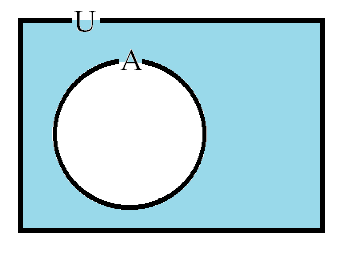
\includegraphics[width=0.3\textwidth]{complement}~
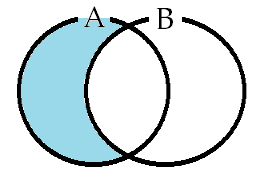
\includegraphics[width=0.3\textwidth]{setminus}

\(A^C\qquad\qquad\qquad\qquad A-B\)
\end{center}
이다.
\end{mdframed}

%
\kswrapfig[Pos=r]{complement_example}{
\exam{}
전체집합 \(U=\{1,2,3,4,5,6\}\)의 두 부분집합 \(A=\{1,3,5\}\), \(B=\{2,3,4\}\)에 대하여 
\begin{align*}
A^C&=\{2,4,6\}\\
A-B&=\{1,5\}\\
B-A&=\{2,4\}
\end{align*}
}

%
\kswrapfig[Pos=r]{complement_problem}{
\prob{}
전체집합 \(U=\{1,2,4,8,16,20\}\)의 두 부분집합 \(A\), \(B\)에 대하여
\begin{align*}
A\cup B&=\{1,2,4,8,16\}\\
A\cap B&=\{1\}\\
A-B&=\{2,4\}
\end{align*}
일 때 오른쪽 벤 다이어그램을 채우고, \(A^C\)와 \(B-A\)를 구하여라.
\par\bigskip\noindent
\(A^C=\)
\par\noindent
\(B-A=\)
}

%
\prob{}
전체집합 \(U=\{x\ba-2\le x\le8\}\)의 두 부분집합
\[A=\{x\ba-2\le x\le4\},\quad B=\{x\ba0<x<7\}\]
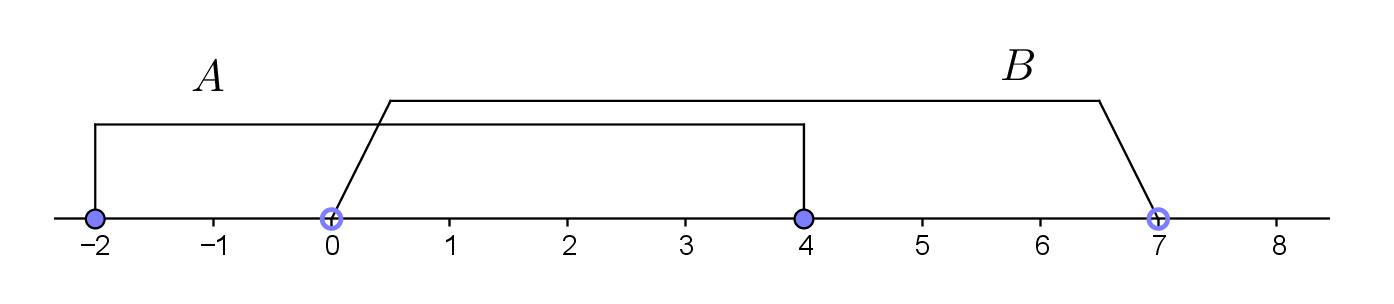
\includegraphics[width=0.9\textwidth]{number_line}

에 대하여 다음을 구하여라.
\begin{enumerate}
\item
\(A^C=\)
\item
\(A-B=\)
\item
\(A-B^C=\)
\end{enumerate}

\clearpage
\begin{mdframed}
%
\defi{서로소}
두 집합 \(A\)와 \(B\)에 대해, \(A\)와 \(B\)가 공통된 원소를 가지고 있지 않으면, 즉
\[A\cap B=\varnothing\]
이면, `\(A\)와 \(B\)가 \textbf{서로소}'라고 한다.
\end{mdframed}

%
\exam{}
\begin{enumerate}
\item
두 집합 \(A=\{2,3,5,7\}\)와 \(B=\{4,6,8,9\}\)에 대하여 \(A\cap B=\varnothing\)이므로 \(A\)와 \(B\)는 서로소이다.
\item
어느 버스에 타고 있는 남자의 집합을 \(A\), 여자의 집합을 \(B\)라고 하면 \(A\cap B=\varnothing\)이므로 \(A\)와 \(B\)는 서로소이다.
\end{enumerate}

%
\prob{}
전체집합 \(U\)와 두 부분집합 \(A\), \(B\)에 대하여 다음 중 두 집합이 서로소인 것을 모두 찾아라.
(단, \(A\neq\varnothing\), \(B\neq\varnothing\))
\par\bigskip\noindent
(1)\:\(A\)와 \(A^C\)
\tabto{0.5\textwidth}
(2)\:\(A\cup B\)와 \(A\)
\par\bigskip\noindent
(3)\:\(A-B\)와 \(B\)
\tabto{0.5\textwidth}
(4)\:\(A-B\)와 \(B-A\)

%
\prob{}
다음 세 집합 \(A\), \(B\), \(C\)에 대하여 서로소인 두 집합을 모두 찾아라.
\[
A=\{x\ba0\le x<2\},\quad
B=\{x\ba x<0\},\quad
C=\{x\ba(x-1)(x-3)\le0\}\]

%%
\section{집합의 원소의 개수}
\begin{mdframed}
%
\defi{집합의 원소의 개수}
집합 \(A\)의 원소의 개수를 기호로
\[n(A)\]
로 나타낸다.
\end{mdframed}

%
\exam{}
\(A=\{1,2,5\}\), \(B=\{1,2,3,\cdots,100\}\), \(C=\varnothing\)이면 \(n(A)=3\), \(n(B)=100\), \(n(C)=0\)이다.

%
\exam{}
\(N=\{x\ba x\text{는 자연수}\}\), \(R=\{x\ba x\text{는 실수}\}\)의 경우, 원소의 개수가 셀 수 없이 많다.
이런 집합에 대해서는 원소의 개수를 생각하지 않는다.
%따라서 \(n(N)\)이나 \(n(R)\)와 같은 기호는 쓰지 않는다.

\kswrapfig[Pos=r]{number_example}{
%
\exam{}
두 집합 \(A=\{3,4,5,6,7\}\), \(B=\{1,3,5\}\)에 대해 \(A\cap B=\{3,5\}\), \(A\cup B=\{1,3,4,5,6,7\}\)이다.
따라서
\begin{align*}
n(A)			&=5\\
n(B)			&=3\\
n(A\cap B)	&=2\\
n(A\cup B)	&=6
\end{align*}
이다.}
이때

\[n(A\cup B)=6=5+3-2=n(A)+n(B)-n(A\cap B)\]
이다.

\begin{mdframed}
%
\theo{}
두 집합 \(A\), \(B\)에 대해
\[n(A\cup B)=n(A)+n(B)-n(A\cap B)\]
이다.
\end{mdframed}

%
\prob{}
다음 값을 구하여라.
\begin{enumerate}
\item
\(n(A)=7\), \(n(B)=4\), \(n(A\cap B)=3\)일 때, \(n(A\cup B)\)의 값
\item
\(n(A)=5\), \(n(B)=11\), \(n(A\cup B)=13\)일 때, \(n(A\cap B)\)의 값
\end{enumerate}

\clearpage
%
\prob{}
어느 컴퓨터 동호회 회원 \(40\)명 중 데스크톱을 가진 회원이 16명, 노트북을 가진 회원이 25명이고, 두 가지 모두 가진 회원이 6명이라고 한다.
데스크톱 또는 노트북을 가진 회원 수를 구하여라.

\begin{mdframed}
전체 컴퓨터 동호회 회원의 집합을 \(U\), 데스크톱을 가진 회원의 집합을 \(A\), 노트북을 가진 회원의 집합을 \(B\)라고 하면
\[n(U)=40,\quad n(A)=16,\quad n(B)=25,\quad n(A\cap B)=6\]
이므로
\[n(A\cup B)=n(A)+n(B)-n(A\cap B)=16+25-6=35\]
이다.
따라서 데스크톱 또는 노트북을 가진 회원 수는 \(35\)명이다.
\end{mdframed}
{\par
\raggedleft\textbf{답 : (\qquad\qquad35명\qquad\qquad)}
\par}

%
\prob{}
어느 회사에서 올 여름 휴가 때에 다녀온 곳을 국내, 국외로 나누어 조사하였다.
직원 \(60\)명 중에서 국내 여행을 다녀온 직원은 36명, 국외 여행을 다녀온 직원은 30명, 두 곳을 모두 다녀온 직원은 18명일 때, 어느 곳도 다녀오지 않은 직원의 수를 구하여라.
\begin{mdframed}
\vspace{0.2\textheight}
\end{mdframed}
\ans

\clearpage
%
\exam{}\label{three_set_numbers_example}
집합 \(A\), \(B\), \(C\)에 대해 \(n(A)=15\), \(n(B)=17\), \(n(C)=10\), \(n(A\cap B)=5\), \(n(B\cap C)=3\), \(n(A\cap C)=2\), \(n(A\cap B\cap C)=1\)이다.
\(n(A\cup B\cup C)\)의 값을 구하여라.

\begin{mdframed}
아래 그림에서
\begin{equation}\label{eq1}
n(A\cup B\cup C)=n(A-B)+n(B-C)+n(C-A)+n(A\cap B\cap C)
\end{equation}
이다.
\par
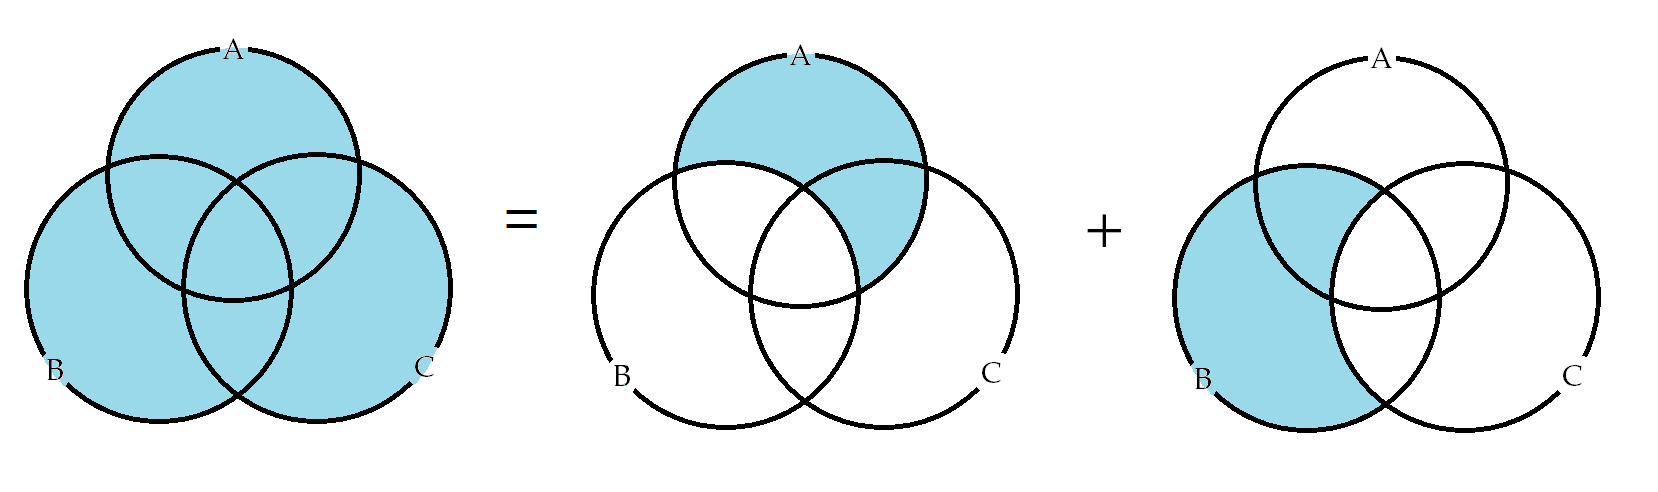
\includegraphics[width=.9\textwidth]{three_set_numbers_1}
\par\vspace{-10pt}
\(\quad n(A\cup B\cup C)\qquad\qquad\quad n(A-B)
\qquad\qquad\qquad n(B-C)\)
\par
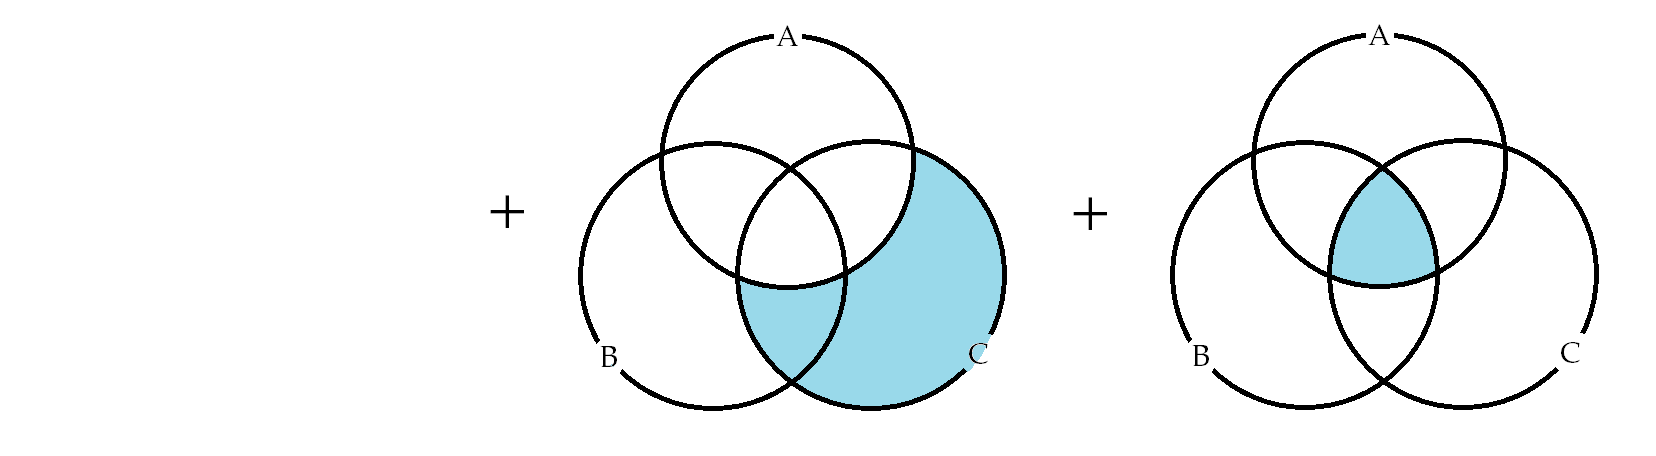
\includegraphics[width=.9\textwidth]{three_set_numbers_2}
\par\vspace{-10pt}
\(\qquad\qquad\qquad\qquad\qquad\quad\:\: n(B-C)
\qquad\qquad\quad\:\: n(A\cap B\cap C)\)
\par
또 \(n(A-B)=n(A)-n(A\cap B)\)이고, 마찬가지로
\par
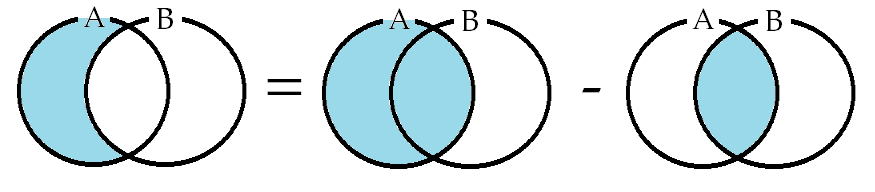
\includegraphics[width=.9\textwidth]{three_set_numbers_3}
\par\vspace{-10pt}
\(\qquad n(A-B)\qquad\qquad\qquad\:\:\: n(A)
\qquad\qquad\qquad\quad\:n(A\cap B)\)
\begin{equation}\label{eq2}
\begin{aligned}
n(A-B)&=n(A)-n(A\cap B)=15-5=10\\
n(B-C)&=n(B)-n(B\cap C)=17-3=14\\
n(C-A)&=n(C)-n(C\cap A)=10-2=8
\end{aligned}
\end{equation}
따라서
\(n(A\cup B\cup C)=n(A-B)+n(B-C)+n(C-A)+n(A\cap B\cap C)=10+14+8+1=33\)
\end{mdframed}
{\par
\raggedleft\textbf{답 : (\qquad\qquad33\qquad\qquad)}
\par}


\begin{mdframed}
%
\theo{}
세 집합 \(A\), \(B\), \(C\)에 대해
\begin{multline*}
n(A\cup B\cup C)=n(A)+n(B)+n(C)\\
-n(A\cap B)-n(B\cap C)-n(C\cap A)+n(A\cap B\cap C)
\end{multline*}
이다.
\end{mdframed}

\proo
예시 \ref{three_set_numbers_example}의 식 (\ref{eq1}), (\ref{eq2})를 사용하면
\begin{align*}
n(A\cup B\cup C)
\stackrel{(\ref{eq1})}=&n(A-B)+n(B-C)+n(C-A)+n(A\cap B\cap C)\\
\stackrel{(\ref{eq2})}=&(n(A)-n(A\cap B))+(n(B)-n(B\cap C))+(n(C)-n(C\cap A))\\
&+n(A\cap B\cap C)\\
=&n(A)+n(B)+n(C)\\
&-n(A\cap B)-n(B\cap C)-n(C\cap A)+n(A\cap B\cap C)
\end{align*}

%
\exam{}
\(K\) 중학교 학생을 대상으로 \(a\), \(b\), \(c\) 세 종류의 책을 읽었는가를 조사하였더니 그 결과가 다음과 같았다.
\par\bigskip\noindent
\(a\)를 읽은 학생 : 28명,				\tabto{0.5\textwidth}\(b\)를 읽은 학생 : 30명,
\par\noindent
\(c\)를 읽은 학생 : 42명,				\tabto{0.5\textwidth}\(a\), \(b\)를 모두 읽은 학생 : 8명,
\par\noindent
\(b\), \(c\)를 모두 읽은 학생 : 5명,		\tabto{0.5\textwidth}\(c\), \(a\)를 모두 읽은 학생 : 10명,
\par\noindent
\(a\), \(b\), \(c\)를 모두 읽은 학생 : 3명
\par\medskip\noindent
이때, \(a\), \(b\), \(c\) 중 적어도 하나를 읽은 학생은 몇 명인가?
\begin{mdframed}
\vspace{0.1\textheight}
\end{mdframed}
\ans

%%
\section{교집합과 합집합의 성질}

%
\exam{}\label{comm}
두 집합 \(A=\{1,2,3,4\}\), \(B=\{1,3,5,7,9\}\)에 대하여 \(A\cap B\)와 \(B\cap A\)를 각각 구해보면
\begin{align*}
A\cap B&=\{1,3\}\\
B\cap A&=\{1,3\}
\end{align*}
이다.
따라서
\[A\cap B=B\cap A\]
이다.
또 \(A\cup B\)와 \(B\cup B\)를 각각 구해보면
\begin{align*}
A\cup B&=\{1,2,3,4,5,7,9\}\\
B\cup A&=\{1,2,3,4,5,7,9\}
\end{align*}
따라서
\[A\cup B=B\cup A\]
이다.
즉, \(A\)와 \(B\)를 교환해도 그 결과는 같다.

\clearpage
%
\prob{}\label{assoc_and_dist}
세 집합 \(A\), \(B\), \(C\)에 대하여 다음 등식이 성립함을 벤 다이어그램을 이용하여 확인하여라.
\begin{enumerate}
\item
\((A\cap B)\cap C=A\cap(B\cap C)\)
\begin{mdframed}[skipabove=0pt,innertopmargin=5pt]
좌변과 우변을 각각 벤 다이어그램으로 표현하면
\par
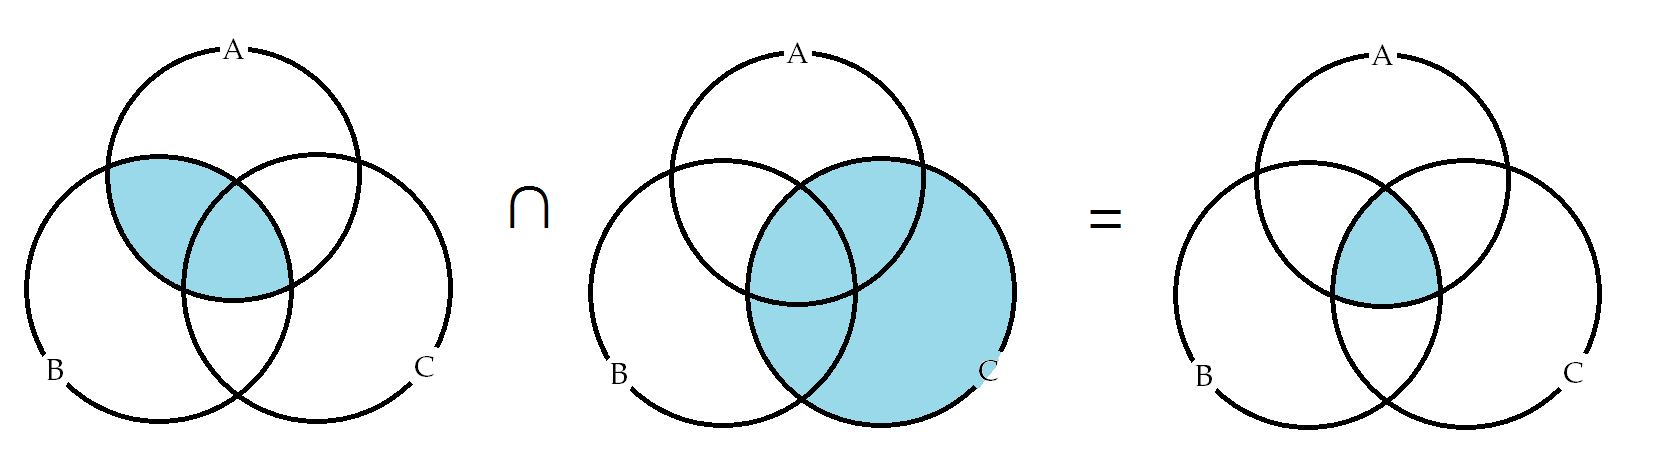
\includegraphics[width=.9\textwidth]{associative_rule_1}
\par\vspace{-10pt}
\(\qquad\:A\cap B\qquad\qquad\qquad\quad\:\:C
\qquad\qquad\qquad\:\:(A\cap B)\cap C\)
\par
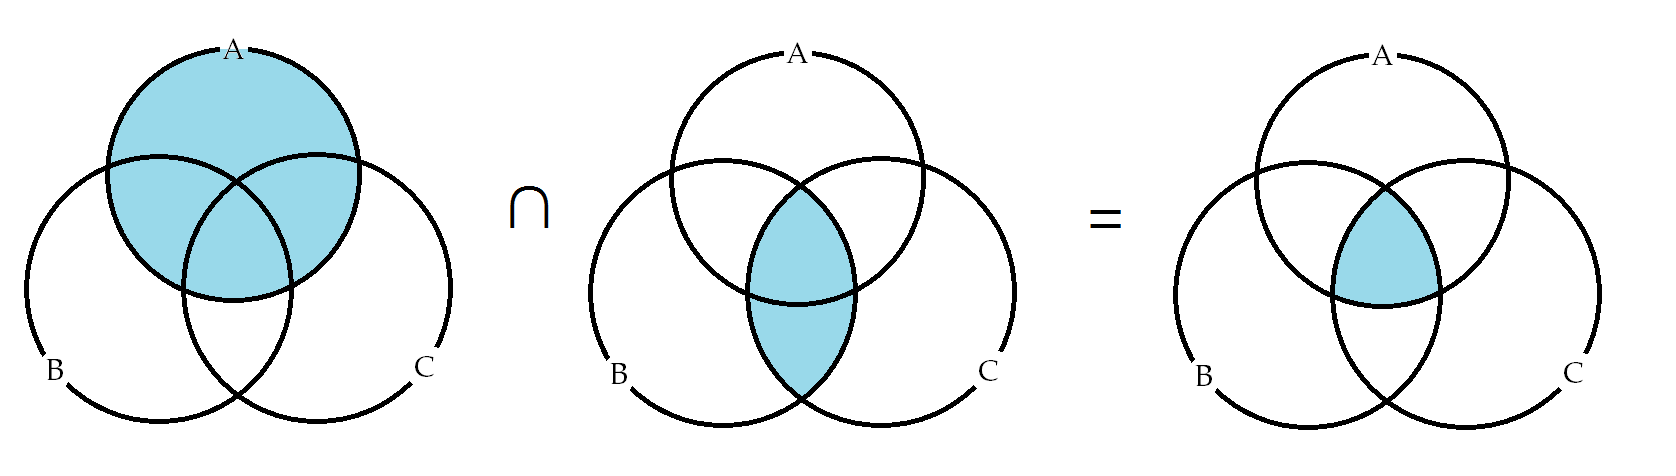
\includegraphics[width=.9\textwidth]{associative_rule_2}
\par\vspace{-10pt}
\(\qquad\quad A\qquad\qquad\qquad\quad\:\:B\cap C
\qquad\qquad\quad\:\: A\cap (B\cap C)\)
\par
이다.
따라서 좌변과 우변이 같다.
\end{mdframed}
%
\item
\((A\cup B)\cup C=A\cup(B\cup C)\)
\begin{mdframed}[skipabove=0pt,innertopmargin=5pt]
좌변과 우변을 각각 벤 다이어그램으로 표현하면
\par
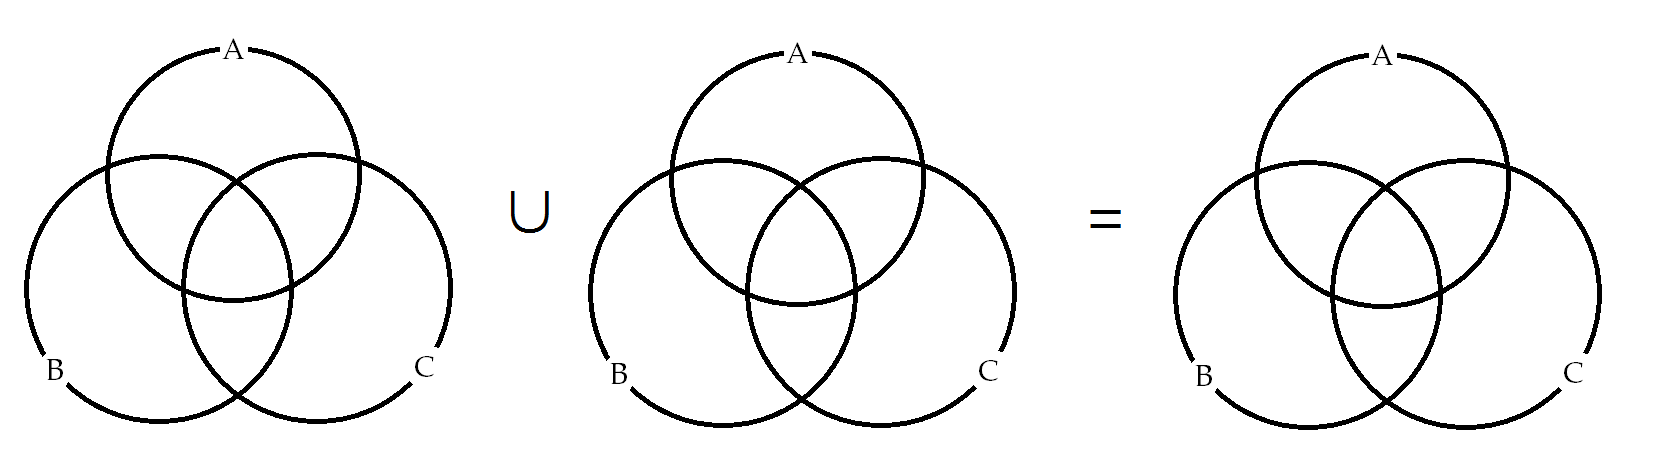
\includegraphics[width=.9\textwidth]{three_set_rule_cup}
\par\vspace{-10pt}
\(\qquad\:A\cup B\qquad\qquad\qquad\quad\:\:C
\qquad\qquad\qquad\:\:(A\cup B)\cup C\)
\par
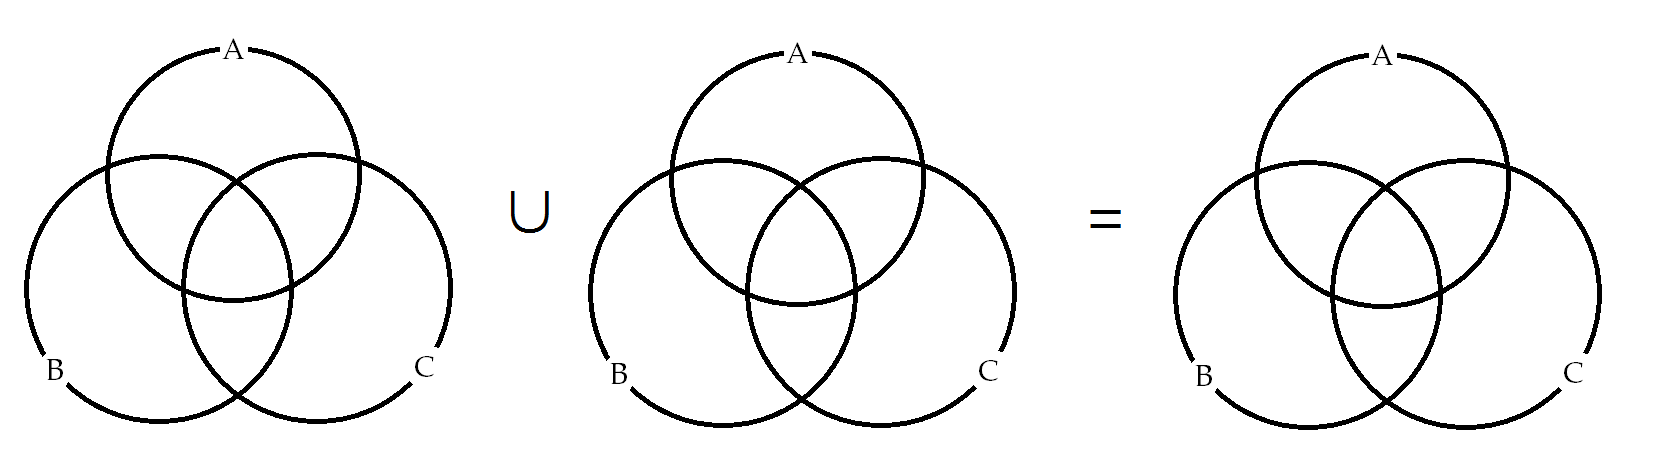
\includegraphics[width=.9\textwidth]{three_set_rule_cup}
\par\vspace{-10pt}
\(\qquad\quad A\qquad\qquad\qquad\quad\:\:B\cup C
\qquad\qquad\quad\:\: A\cup (B\cup C)\)
\par
이다.
따라서 좌변과 우변이 같다.
\end{mdframed}
%
\item
\(A\cap(B\cup C)=(A\cap B)\cup(A\cap C)\)
\begin{mdframed}[skipabove=0pt,innertopmargin=5pt]
좌변과 우변을 각각 벤 다이어그램으로 표현하면
\par
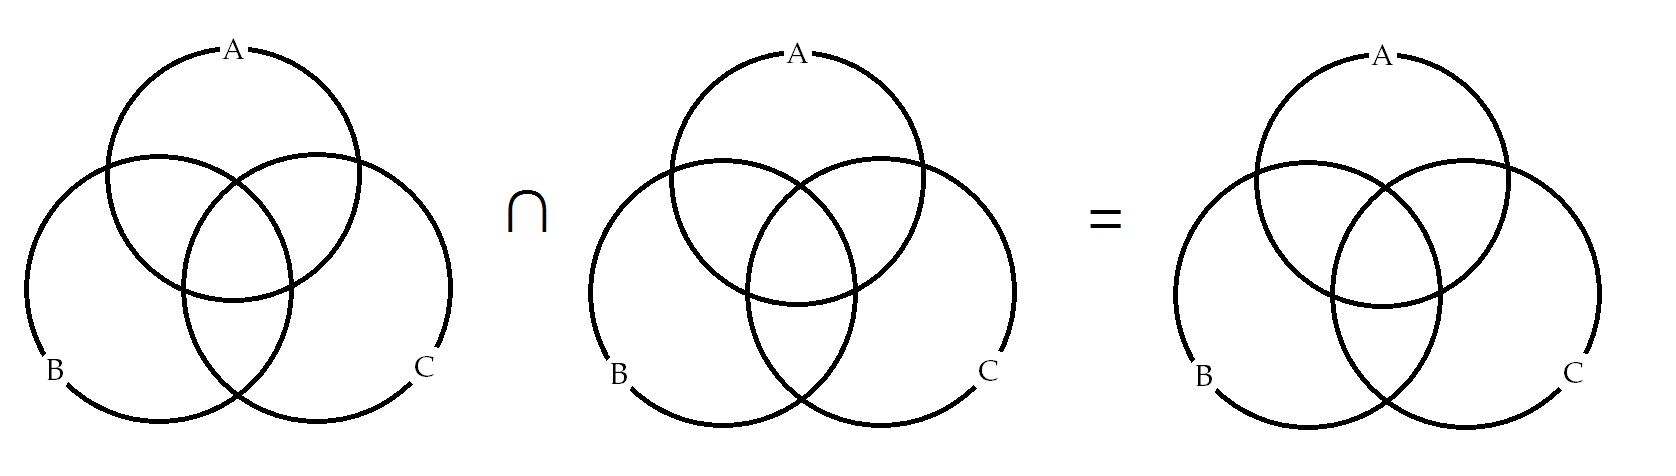
\includegraphics[width=.9\textwidth]{three_set_rule_cap}
\par\vspace{-10pt}
\(\qquad\quad\:A\qquad\qquad\qquad\quad\:\:B\cup C
\qquad\qquad\quad\:A\cap(B\cup C)\)
\par
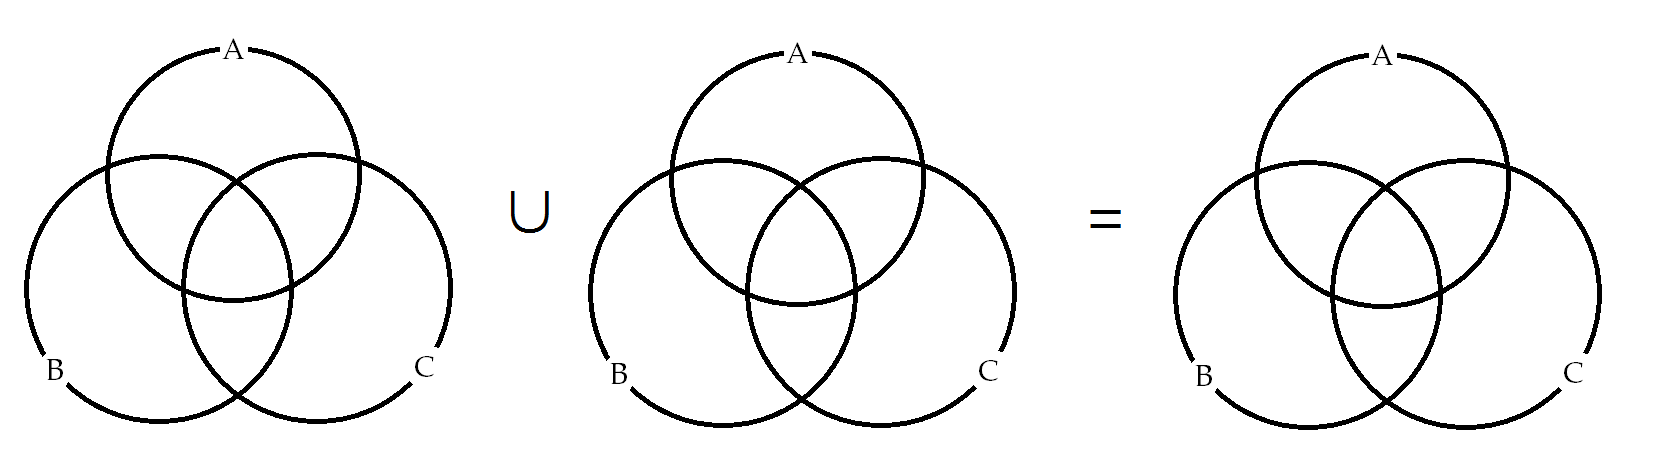
\includegraphics[width=.9\textwidth]{three_set_rule_cup}
\par\vspace{-10pt}
\(\qquad A\cap B\qquad\qquad\qquad\:\:A\cap C
\qquad\qquad(A\cap B)\cup(A\cap C)\)
\par
이다.
따라서 좌변과 우변이 같다.
\end{mdframed}
%
\item
\(A\cup(B\cap C)=(A\cup B)\cap(A\cup C)\)
\begin{mdframed}[skipabove=0pt,innertopmargin=5pt]
좌변과 우변을 각각 벤 다이어그램으로 표현하면
\par
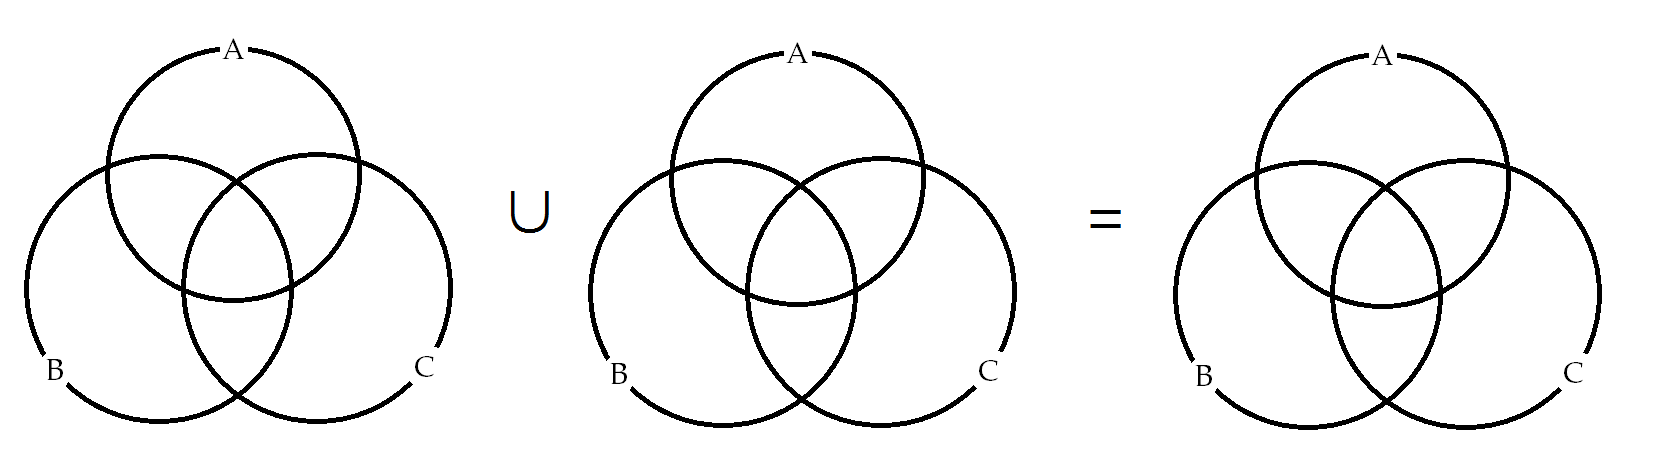
\includegraphics[width=.9\textwidth]{three_set_rule_cup}
\par\vspace{-10pt}
\(\qquad\quad\:A\qquad\qquad\qquad\quad\:\:B\cap C
\qquad\qquad\quad\:A\cup(B\cap C)\)
\par
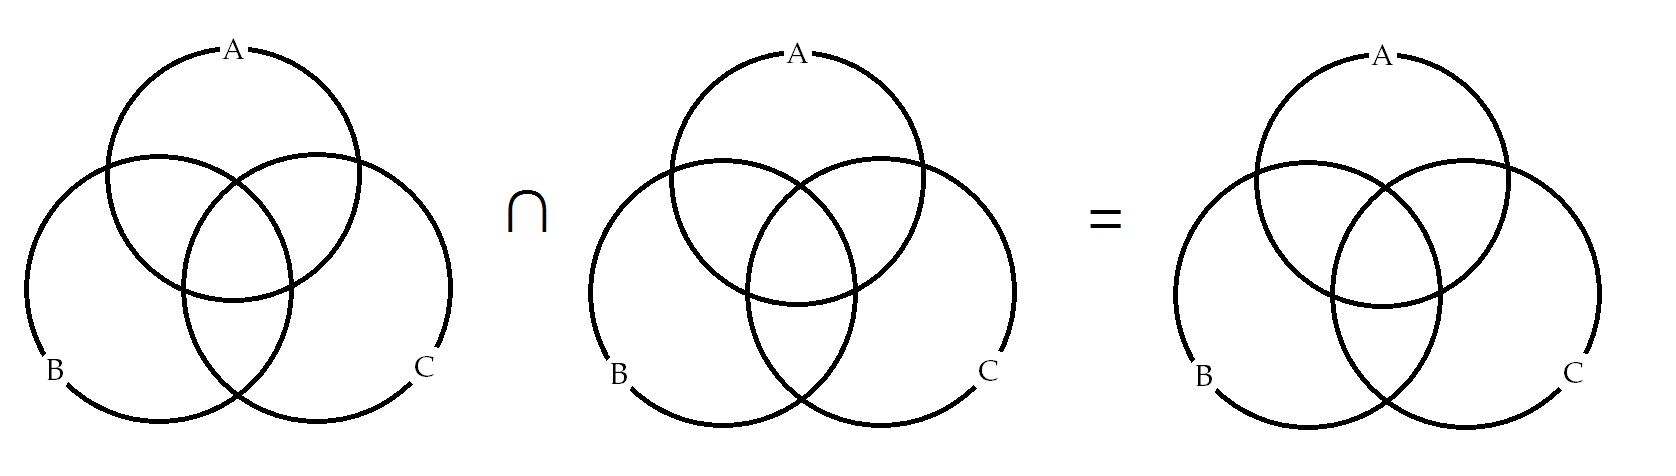
\includegraphics[width=.9\textwidth]{three_set_rule_cap}
\par\vspace{-10pt}
\(\qquad A\cup B\qquad\qquad\qquad\:\:A\cup C
\qquad\qquad(A\cup B)\cap(A\cup C)\)
\par
이다.
따라서 좌변과 우변이 같다.
\end{mdframed}
\end{enumerate}

\clearpage
예제 \ref{comm}와 문제 \ref{assoc_and_dist}를 종합하면 다음 정리를 얻는다.
\begin{mdframed}
%
\theo{집합의 연산법칙}\label{basic_property}
세 집합 \(A\), \(B\), \(C\)에 대해 다음 법칙들이 성립한다.
\begin{enumerate}
\item
교환법칙\\
\(A\cap B=B\cap A\)\\
\(A\cup B=B\cup A\)
\item
결합법칙\\
\((A\cap B)\cap C=A\cap(B\cap C)\)\\
\((A\cup B)\cup C=A\cup(B\cup C)\)
\item
분배법칙\\
\(A\cap(B\cup C)=(A\cap C)\cup(A\cap C)\)\\
\(A\cup(B\cap C)=(A\cup C)\cap(A\cup C)\)
\end{enumerate}
\end{mdframed}

\bigskip\bigskip
다음의 `수의 연산법칙'과 비교하여 기억하자.

\begin{mdframed}
%
\theo{수의 연산법칙}
숫자 \(a\), \(b\), \(c\)에 대해 다음 법칙들이 성립한다.
\begin{enumerate}
\item
교환법칙\\
\(a+b=b+a\)\\
\(a\times b=b\times a\)
\item
결합법칙\\
\((a+b)+c=a+(b+c)\)\\
\((a\times b)\times c=a\times(b\times c)\)
\item
분배법칙\\
\(a\times(b+c)=a\times b+a\times c\)
\end{enumerate}
\end{mdframed}
%이 법칙은 모든 종류의 수(자연수, 정수, 유리수, 실수, 복소수)에 적용가능하다.

\clearpage
%
\prob{}
차집합에 대한 교환법칙과 결합법칙은 성립하는지 확인하여라.
\begin{align*}
교환법칙\:&:\:A-B=B-A\\
결합법칙\:&:\:A-(B-C)=(A-B)-C
\end{align*}

\begin{mdframed}[skipabove=0pt,innertopmargin=5pt]
교환법칙 :
\par
\begin{center}
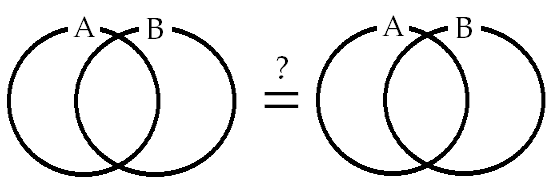
\includegraphics[width=.5\textwidth]{two_set_equality}
\par\(A-B\qquad\qquad\qquad\:\:B-A\)
\end{center}
\par\bigskip\noindent
결합법칙 :
\par
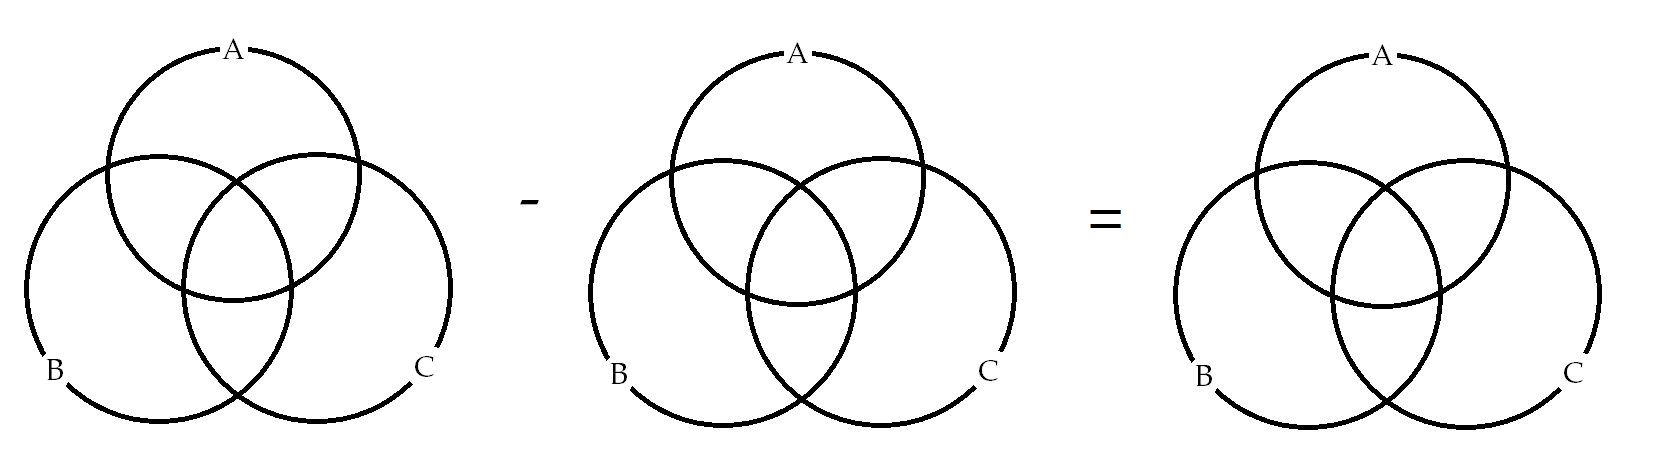
\includegraphics[width=.9\textwidth]{three_set_rule_setminus}
\par\vspace{-10pt}
\(\qquad\quad\:A\qquad\qquad\qquad\qquad B-C
\qquad\qquad\qquad\:A-(B-C)\)
\par
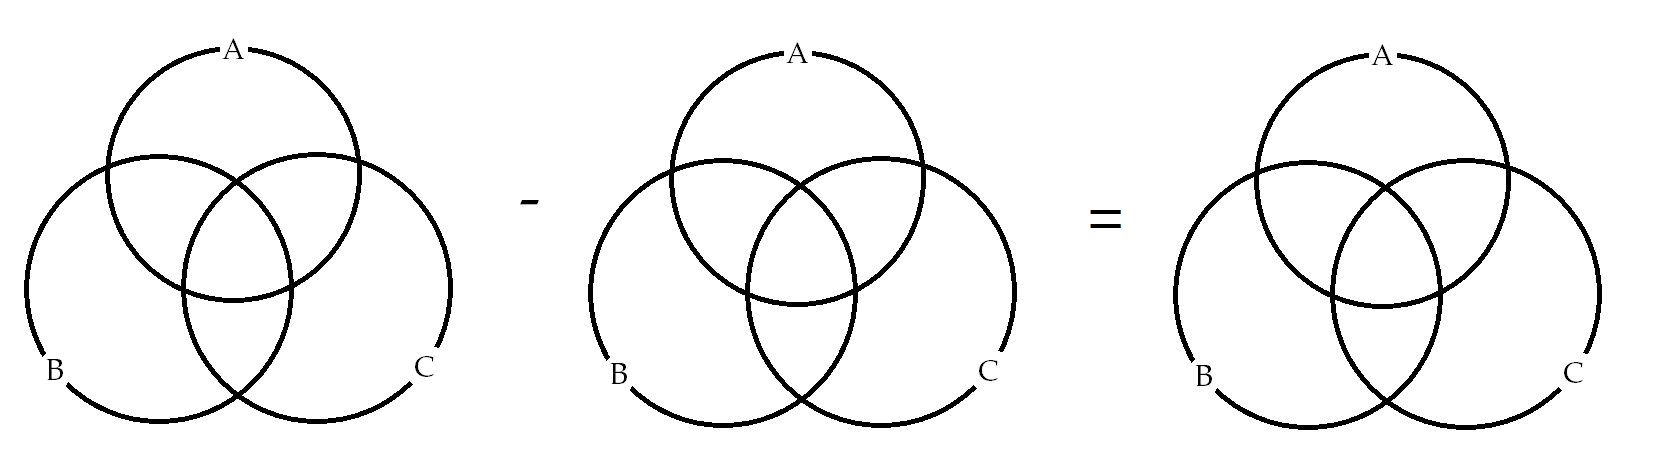
\includegraphics[width=.9\textwidth]{three_set_rule_setminus}
\par\vspace{-10pt}
\(\qquad A-B\qquad\qquad\qquad\qquad\:\: C
\qquad\qquad\qquad\quad(A-B)-C\)
\par
\end{mdframed}
{\par\bigskip
\raggedleft\textbf{답 :}
교환법칙이 (성립한다 / 성립하지 않는다.)\par
결합법칙이 (성립한다 / 성립하지 않는다.)
\par}
\clearpage
%
\prob{흡수법칙}\label{absorb}
두 집합 \(A\), \(B\)에 대하여 다음 등식이 성립함을 벤 다이어그램을 이용하여 확인하여라.
\begin{enumerate}
\vspace{-5pt}\item
\(A\cup (A\cap B)=A\)
\begin{mdframed}[skipabove=0pt,innertopmargin=5pt]
좌변을 벤 다이어그램으로 표현하면
\par
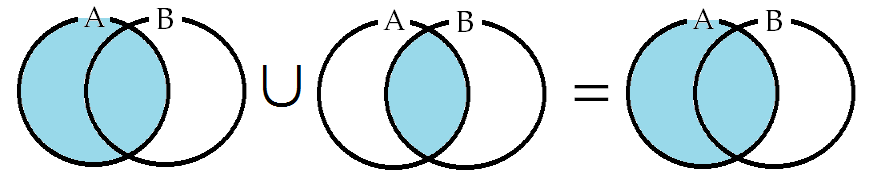
\includegraphics[width=.9\textwidth]{absorption_rule}
\par\vspace{-10pt}
\(\qquad\quad\:\:A\qquad\qquad\qquad\quad\:\:\:A\cap B
\qquad\qquad\quad\:\:A\cup (A\cap B)\)
\par
이다.
따라서 우변인 \(A\)와 같다.
\end{mdframed}
%
\item
\(A\cap (A\cup B)=A\)
\begin{mdframed}[skipabove=0pt,innertopmargin=5pt]
좌변을 벤 다이어그램으로 표현하면
\par
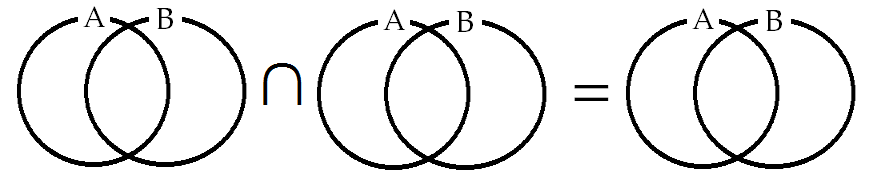
\includegraphics[width=.9\textwidth]{two_set_rule_cap}
\par\vspace{-10pt}
\(\qquad\quad\:\:A\qquad\qquad\qquad\quad\:\:\:A\cup B
\qquad\qquad\quad\:\:A\cap (A\cup B)\)
\par
이다.
따라서 우변인 \(A\)와 같다.
\end{mdframed}
\end{enumerate}

%
\prob{}
세 집합 \(A\), \(B\), \(C\)에 대하여 \(A\)와 \(B\)가 서로소일 때, 다음 등식이 성립함을 벤 다이어그램을 이용하여 확인하여라.
\[A\cap(B\cup C)=A\cap C\]
\vspace{-15pt}
\begin{mdframed}
\(A\)와 \(B\)가 서로소인 것을 감안해 벤 다이어그램을 그리고 좌변을 표현하면
\par\vspace{5pt}
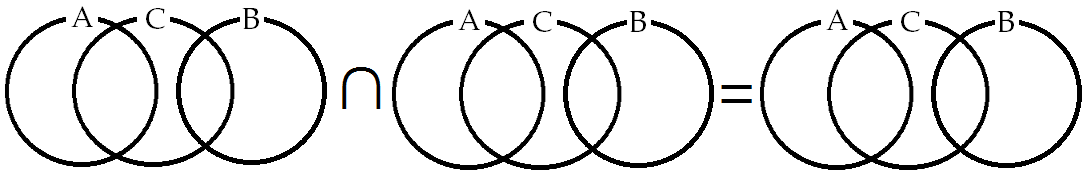
\includegraphics[width=.9\textwidth]{disjoint_A_and_B_cap}
\par\(\qquad\qquad A\qquad\qquad\qquad\qquad\:\: B\cup C
\qquad\qquad\quad\:\:A\cap(B\cup C)\)
\par
이다. 따라서 우변인 \(A\cap C\)와 같다.
\end{mdframed}

%%
\section{여집합과 차집합의 성질}

%
\prob{}\label{setminus}
두 집합 \(A\), \(B\)에 대하여 다음 등식이 성립함을 벤 다이어그램을 이용하여 확인하여라.
\[A\cap B^C=A-B\]
\begin{mdframed}[skipabove=0pt,innertopmargin=5pt]
좌변을 벤 다이어그램으로 표현하면
\par
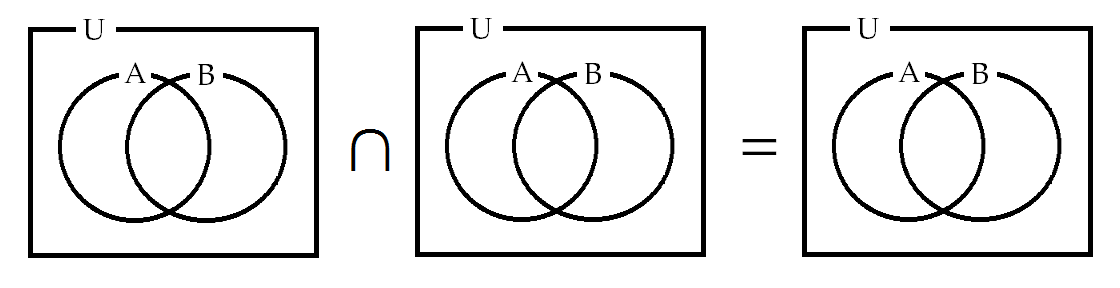
\includegraphics[width=.9\textwidth]{two_set_rule-cap}
\par\vspace{-10pt}
\(\qquad\qquad A\qquad\qquad\qquad\qquad\quad\:B^C
\qquad\qquad\qquad\quad\:\:A\cap B^C\)
\par\noindent
이다.
따라서 우변인 \(A-B\)와 같다.
\end{mdframed}

%
\prob{}
두 집합 \(A\), \(B\)에 대하여 다음 등식이 성립함을 벤 다이어그램을 이용하여 확인하여라.
\[(A-B)\cup(B-A)=(A\cup B)-(A\cap B)\]
\begin{mdframed}[skipabove=0pt,innertopmargin=5pt]
좌변을 벤 다이어그램으로 표현하면
\par
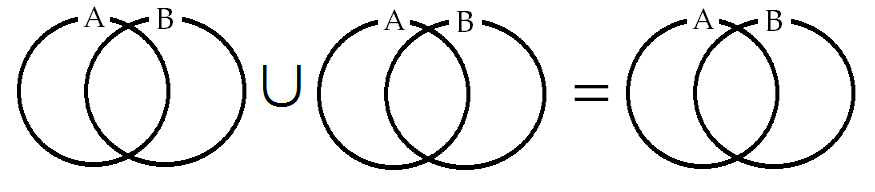
\includegraphics[width=.9\textwidth]{two_set_rule_cup}
\par\vspace{-10pt}
\(\qquad\quad A-B\qquad\qquad\qquad\quad B-A
\qquad\qquad\quad(A-B)\cup(B-A)\)
\par
이고 우변을 벤 다이어그램으로 표시하면
\par
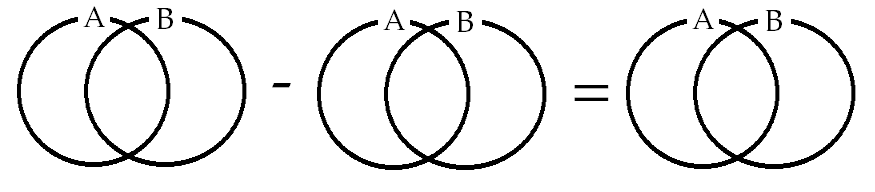
\includegraphics[width=.9\textwidth]{two_set_rule_setminus}
\par\vspace{-10pt}
\(\qquad\quad A\cup B\qquad\qquad\qquad\quad\: A\cap B
\qquad\qquad\quad(A\cup B)-(A\cap B)\)
\par
이다.
따라서 좌변과 우변은 같다.
\end{mdframed}

%
\prob{}
세 집합 \(A\), \(B\), \(C\)에 대하여 다음 등식이 성립함을 벤 다이어그램을 이용하여 확인하여라.
\[A-(B\cap C)=(A-B)\cup(A-C)\]
\begin{mdframed}[skipabove=0pt,innertopmargin=5pt]
좌변을 벤 다이어그램으로 표현하면
\par
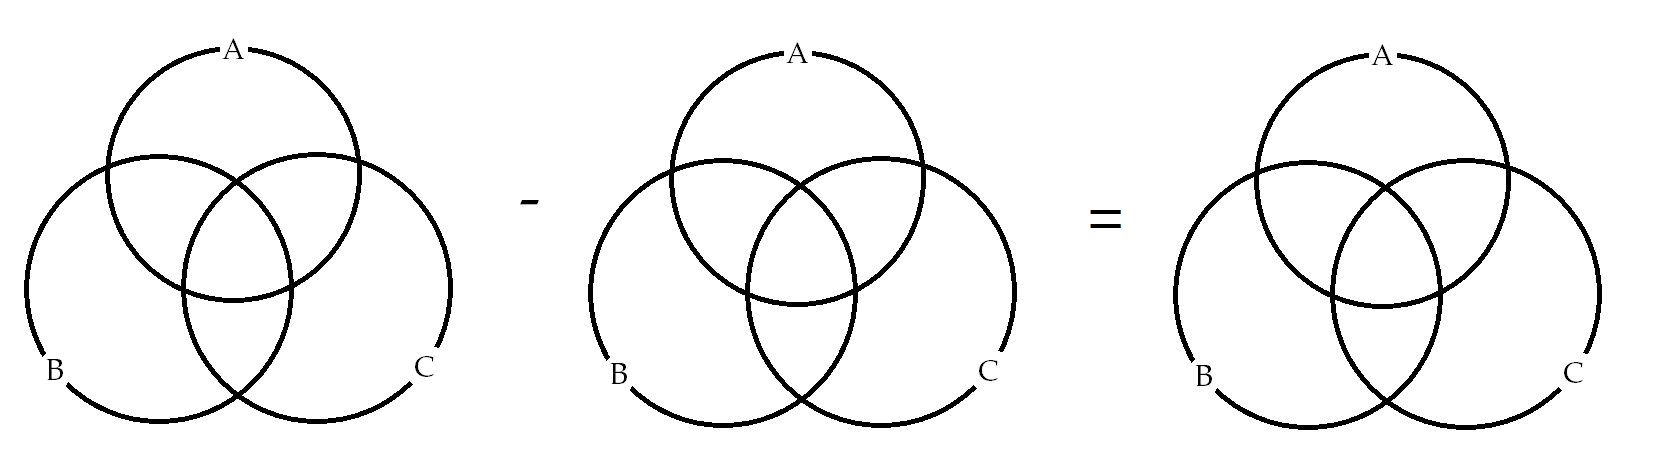
\includegraphics[width=.9\textwidth]{three_set_rule_setminus}
\par\vspace{-10pt}
\(\qquad\quad\:\: A\qquad\qquad\qquad\qquad\: B\cap C
\qquad\qquad\qquad A-(B\cap C)\)
\par
이고 우변을 벤 다이어그램으로 표시하면
\par
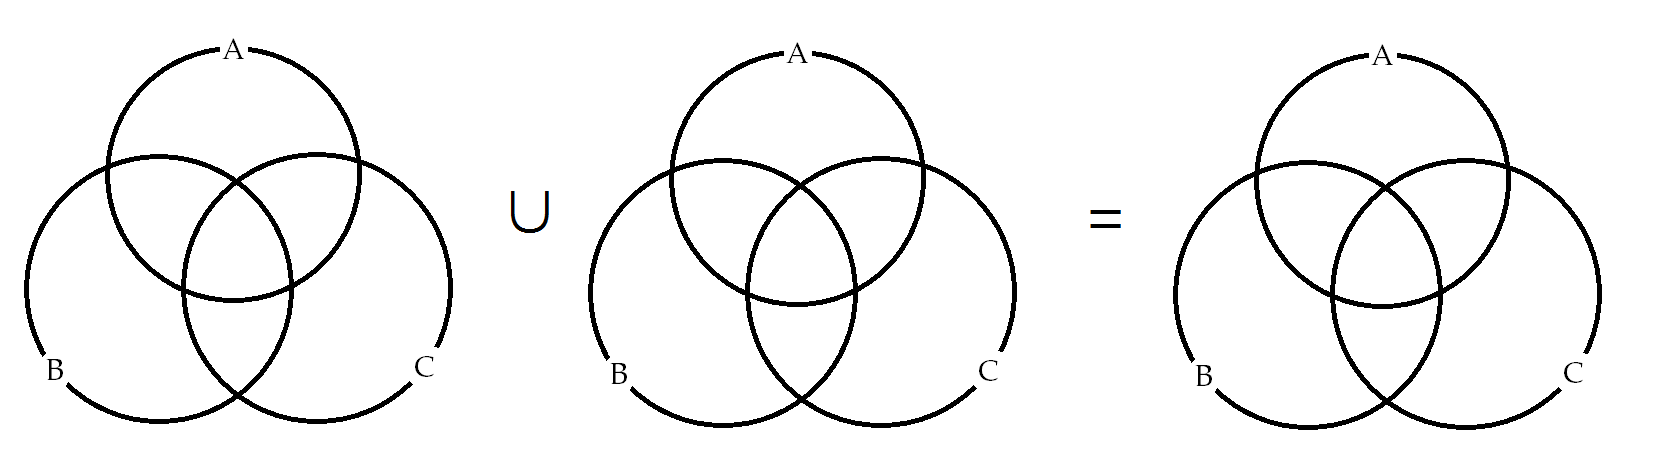
\includegraphics[width=.9\textwidth]{three_set_rule_cup}
\par\vspace{-10pt}
\(\qquad\:\:A-B\qquad\qquad\qquad\quad\:A-C
\qquad\qquad\:\:(A-B)\cup(A-C)\)
\par
이다.
따라서 좌변과 우변은 같다.
\end{mdframed}

\clearpage
%
\kswrapfig[Pos=r]{one_set_rule}{
\prob{}
전체집합 \(U\)의 부분집합 \(A\)에 대하여 다음 등식이 성립함을 벤 다이어그램을 이용하여 확인하여라.
}
\begin{enumerate}
\item
\((A^C)^C=A\)
\item
\(A\cup A^C=U\)
\item
\(A\cap A^C=\varnothing\)
\end{enumerate}

%
이상에서 여집합과 차집합에 대하여 다음 등식이 성립함을 알 수 있다.
\begin{mdframed}
%
\theo{여집합과 차집합의 성질}\label{complement_property}
\begin{enumerate}
\item
\(U^C=\varnothing\), \(\varnothing^C=U\)
\item
\(A-B=A\cap B^C\)
\item
\((A^C)^C=A\)
\item
\(A\cap A^C=\varnothing\), \(A\cup A^C=U\)
\item
\((A-B)\cup(B-A)=(A\cup B)-(A\cap B)\)
\item
\(A-(B\cap C)=(A-B)\cup(A-C)\)
\end{enumerate}
\end{mdframed}

\clearpage
%
\prob{}\label{de_morgan_proof}
두 집합 \(A\), \(B\)에 대하여 다음 등식이 성립함을 벤 다이어그램을 이용하여 확인하여라.
\begin{enumerate}
\item
\((A\cap B)^C=A^C\cup B^C\)
\begin{mdframed}[skipabove=0pt,innertopmargin=5pt]
좌변과 우변을 각각 벤 다이어그램으로 표현하면
\par
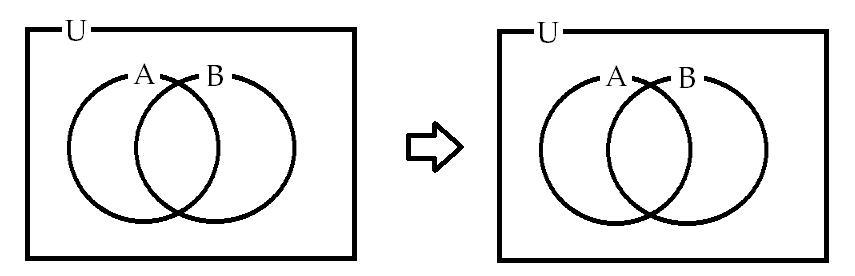
\includegraphics[width=.9\textwidth]{two_set_rule-complement}
\par\vspace{-10pt}
\(\qquad\qquad\:\: A\cap B\qquad\qquad\qquad\qquad\qquad\quad\:\:(A\cap B)^C\)
\par
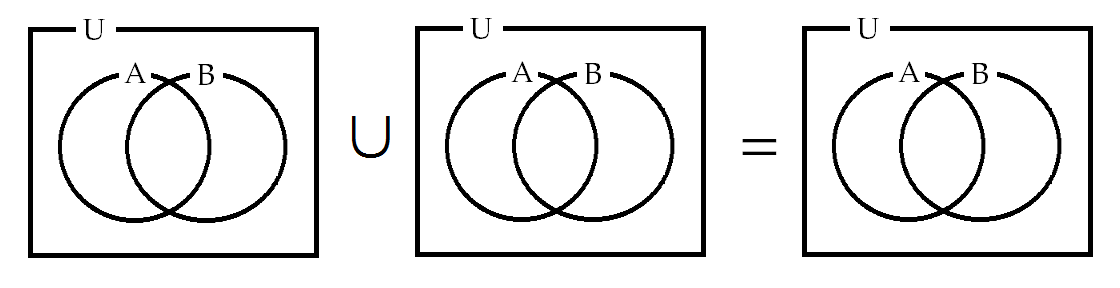
\includegraphics[width=.9\textwidth]{two_set_rule-cup}
\par\vspace{-10pt}
\(\qquad\quad\:\:A^C\qquad\qquad\qquad\qquad B^C
\qquad\qquad\qquad A^C\cup B^C\)
\par
이다.
따라서 좌변과 우변이 같다.
\end{mdframed}
%
\item
\((A\cup B)^C=A^C\cap B^C\)
\begin{mdframed}[skipabove=0pt,innertopmargin=5pt]
좌변과 우변을 각각 벤 다이어그램으로 표현하면
\par
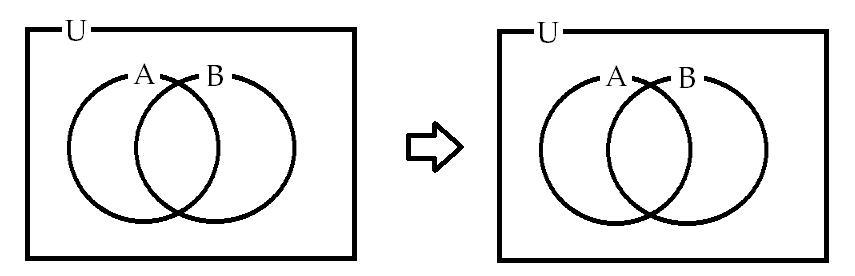
\includegraphics[width=.9\textwidth]{two_set_rule-complement}
\par\vspace{-10pt}
\(\qquad\qquad\:\: A\cup B\qquad\qquad\qquad\qquad\qquad\quad\:\:(A\cup B)^C\)
\par
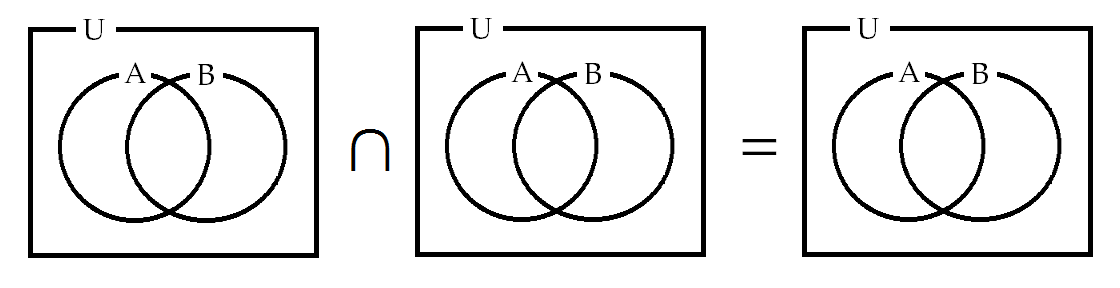
\includegraphics[width=.9\textwidth]{two_set_rule-cap}
\par\vspace{-10pt}
\(\qquad\quad\:\:A^C\qquad\qquad\qquad\qquad B^C
\qquad\qquad\qquad A^C\cap B^C\)
\par
이다.
따라서 좌변과 우변이 같다.
\end{mdframed}
\end{enumerate}

이상을 정리하면 다음 정리를 얻는다.
\begin{mdframed}
%
\theo{드모르간의 법칙}\label{de_morgan}
두 집합 \(A\), \(B\)에 대해
\begin{enumerate}
\item
\((A\cap B)^C=A^C\cup B^C\)
\item
\((A\cup B)^C=A^C\cap B^C\)
\end{enumerate}
\end{mdframed}

%
\prob{}
전체집합 \(U\)의 두 부분집합 \(A\), \(B\)에 대하여, 다음 등식들이 성립함을
%정리 \ref{complement_property}와 드모르간의 법칙(정리 \ref{de_morgan})을 이용하여 확인하여라.
집합의 연산법칙들을 이용하여 확인하여라.
\begin{enumerate}
\item
\((A-B)^C=A^C\cup B\)
\begin{mdframed}
\begin{align*}
(A-B)^C
&=(A\cap B^C)^C&(차집합의 성질)\\
&=A^C\cup(B^C)^C&(드모르간의 법칙)\\
&=A^C\cup B&(여집합의 성질)\\
\end{align*}
\end{mdframed}
\item
\((A-B)-C=A-(B\cup C)\)
\begin{mdframed}
\vspace{0.4\textwidth}
\end{mdframed}
\end{enumerate}

%%
\section{보충·심화 문제}

%
\prob{}
전체집합 \(U=\{1,2,3,4,5,6,7\}\)의 두 부분집합 \(A=\{2,3,4,5\}\), \(B=\{1,3,5,7\}\)에 대하여 다음을 구하여라.
\begin{enumerate}
\item
\(A\cap B=\)
\item
\(A\cup B=\)
\item
\(A-B=\)
\item
\(A^C=\)
\end{enumerate}

%
\prob{}
전체집합 \(U=\{x\ba x\text{는 12 이하의 자연수}\}\)의 세 부분집합
\[
A=\{x\ba x\text{는 짝수}\},\quad
B=\{x\ba x\text{는 4의 배수}\},\quad
C=\{x\ba x\text{는 12의 약수}\}
\]
에 대하여 다음을 구하여라.
\begin{enumerate}
\item
\(A\cap B^C=\)
\item
\((A\cap C)^C=\)
\item
\((A\cap B)\cup C=\)
\item
\((A-B)\cap(A-C)=\)
\end{enumerate}

%
\prob{}
\(A\)와 \(B\)가 서로소일 때, 다음을 간단히 하여라.
\[(A\cap B)\cup C\]
\tabb{A\cap B}{A\cup B}{A\cap C}{A\cup C}C

%
\prob{}
\(A\)와 \(B\)가 서로소일 때, 다음을 간단히 하여라.
\[A\cap (B\cup C)\]
\tabb{A\cap B}{A\cup B}{A\cap C}{A\cup C}C

%
\prob{}
전체집합 \(U=\{1,2,3,\cdots,10\}\)의 두 부분집합
\[A=\{x\ba x\text{는 2의 배수}\},\quad B=\{3,5,7,9\}\]
에 대하여 \(n(A^C\cup B^C)\)를 구하여라.
\tabb6789{10}

%
\prob{}
전체집합 \(U\)의 두 부분집합 \(A\), \(B\)에 대하여 다음 등식이 성립함을 집합의 연산법칙을 사용하여 보여라.
\begin{enumerate}
\item
\((A\cup B)\cap(A^C\cup B)=B\)
\begin{mdframed}
\vspace{0.3\textwidth}
\end{mdframed}
\item
\((A\cap B)\cup(A-B)=A\)
\begin{mdframed}
\vspace{0.3\textwidth}
\end{mdframed}
\item
\((A-B)\cap(B-A)=\varnothing\)
\begin{mdframed}
\vspace{0.3\textwidth}
\end{mdframed}
\item
\(A-(B\cup C)=(A-B)\cap(A-C)\)
\begin{mdframed}
\vspace{0.3\textwidth}
\end{mdframed}
%\item
%\(\left[(A-B)\cup(A\cap C)\right]^C=A^C\cup(B\cap C^C)\)
%\begin{mdframed}
%\vspace{0.3\textwidth}
%\end{mdframed}
\end{enumerate}

%
\prob{}
전체집합 \(U\)의 세 부분집합 \(A\), \(B\), \(C\)에 대하여 다음 등식이 성립함을 벤 다이어그램을 사용하여 보여라.
\[(A\cup B)\cap(A^C\cap B^C)=\varnothing\]
\begin{mdframed}
\vspace{0.4\textwidth}
\end{mdframed}

%
\prob{}
두 집합 \(A=\{a-3,a-1,a\}\), \(B=\{0,2,a^2-3a\}\)에 대하여 \(A\cap B=\{-2,0\}\)일 때, 상수 \(a\)의 값을 구하여라.
\tabb{-2}{-1}012

%
\prob{}
다음 중 \(A\subset B\)인 경우가 아닌 것을 고르시오.
\tabb{A\cap B=A}{A\cup B=A}{A-B=\varnothing}{B^C\subset A^C}{A=B}

%
\prob{}
두 집합 \(A=\{1,2,4,8\}\), \(B=\{2,3,4,5\}\)에 대하여 다음 두 조건을 만족하는 집합 \(X\)의 개수를 구하시오.
\begin{enumerate}
\item
\(A\cap X=X\)
\item
\((A-B)\cup X=X\)
\end{enumerate}
\tabb1248{16}

%
\prob{}
전체집합 \(U=\{2,3,4,5,6\}\)의 두 부분집합 \(A\), \(B\)가 다음 두 조건을 만족한다.
\begin{enumerate}
\item
\(A\cup B=U\)
\item
\(A\cap B=\{2,3,5\}\)
\end{enumerate}
집합 \(X\)의 원소의 합을 \(f(X)\)라고 할 때, \(f(A)\times f(B)\)의 최댓값을 구하여라.

%
\prob{}
60명의 학생을 대상으로 축구와 야구 중 좋아하는 스포츠를 조사하였다.
축구를 좋아하는 학생은 37명이고,
야구를 좋아하는 학생은 42명이며,
축구와 야구를 모두 좋아하는 학생은 \(k\)명일 때,
\(k\)의 최댓값과 최솟값을 구하여라.

%%
\section*{답}

%
\an4
(1) \(A\cap B=\{2,3\}\),		 	\(A\cup B=\{1,2,3,5,6,7\}\)\\
(2) \(A\cap B=\{5\}\),			 	\(A\cup B=\{1,2,3,5,7,8,9\}\)\\
(3) \(A\cap B=\{x\ba1<x\le4\}\), 	\(A\cup B=\{x\ba-3\le x<9\}\)

%
\an9
\(A^C=\{8,16,20\}\)\\
\(B-A=\{8,16\}\)

%
\an{10}
(1) \(A^C=\{x\ba x>4\}\)\\
(2) \(A-B=\{x\ba-2\le x\le0\}\)\\
(3) \(A-B^C=\{x\ba0<x\le4\}\)

%
\an{13}
(1), (3), (4)

%
\an{14}
\(A\)와 \(B\)가 서로소\\
\(B\)와 \(C\)가 서로소

%
\an{21}
(1) \(8\)\\
(2) \(3\)

%
\an{23}
12명

%
\an{26}
80명

%
\an{31}
교환법칙이 성립하지 않는다\\
결합법칙이 성립하지 않는다.

%
\an{42}
(2)
\begin{align*}
(A-B)-C
&=(A\cap B^C)-C			&(\text{차집합의 성질})\\
&=(A\cap B^C)\cap C^C		&(\text{차집합의 성질})\\
&=A\cap(B^C\cap C^C)		&(\text{교집합의 결합법칙})\\
&=A\cap(B\cup C)^C		&(\text{드모르간의 법칙})\\
&=A-(B\cup C)				&(\text{차집합의 성질})
\end{align*}

%
\an{43}
(1) \(\{3,5\}\)\\
(2) \(\{1,2,3,4,5,7\}\)\\
(3) \(\{2,4\}\)\\
(4) \(\{1,6,7\}\)

%
\an{44}
(1) \(\{2,6,10\}\)\\
(2) \(\{1,3,5,7,8,9,10,11\}\)\\
(3) \(\{1,2,3,4,6,8,12\}\)\\
(4) \(\{10\}\)

%
\an{45}
\ding{176}

%
\an{46}
\ding{174}

%
\an{47}
\ding{176}

%
\an{48}
(1)
\begin{align*}
(A\cup B)\cap(A^C\cup B)
&=(B\cup A)\cap(B\cup A^C)	&(\text{합집합의 교환법칙})\\
&=B\cup(A\cap A^C)		&(\text{분배법칙})\\
&=B\cup\varnothing\\
&=B
\end{align*}
\par\noindent
(2)
\begin{align*}
(A\cap B)\cup(A-B)
&=(A\cap B)\cup(A\cap B^C)	&(\text{차집합의 성질})\\
&=A\cap(B\cup B^C)		&(\text{분배법칙})\\
&=A\cup U\\
&=A
\end{align*}
\par\noindent
(3)
\begin{align*}
(A-B)\cap(B-A)
&=(A\cap B^C)\cap(B\cap A^C)	&(\text{차집합의 성질})\\
&=(A\cap A^C)\cap(B\cap B^C)	&(\text{교집합의 결합법칙, 교환법칙})\\
&=\varnothing\cap\varnothing=\varnothing
\end{align*}
\par\noindent
(4)
\begin{align*}
A-(B\cup C)
&=A\cap(B\cup C)^C			&(\text{차집합의 성질})\\
&=A\cap(B^C\cap C^C)			&(\text{드모르간의 법칙})\\
&=(A\cap A)\cap(B^C\cap C^C)		\\
&=(A\cap B^C)\cap(A\cap C^C)	&(\text{교집합의 결합법칙, 교환법칙})\\
&=(A-B)\cap(A-C)				&(\text{차집합의 성질})
\end{align*}

%
\an{49}
생략

%
\an{50}
\ding{175}

%
\an{51}
\ding{173}

%
\an{52}
\ding{174}

%
\an{53}
224

%
\an{54}
최댓값 : 37, 최솟값 : 19
\end{document}